\chapter{Técnicas}

\section{Test-Driven Development}
\label{sub:tdd}
``Apenas escrever código para corrigir um teste falhando". Segundo \citeonline{TestDrivenKoskela}, isto é \textit{Test-Driven Development} (TDD) \cite{TDDbyExample} em apenas uma sentença.

O TDD é uma técnica onde o desenvolvimento do software é guiado por \textbf{testes automatizados}, que são escritos antes de qualquer linha de código. Primeiro escreve-se um teste, depois escreve-se o código para passar neste teste. Em seguida, o código é refatorado para encontrar um design melhor, contanto sempre com os testes existentes para que não sejam introduzidas falhas em outras partes do sistema.

Esta abordagem encoraja bom design \cite{GrowingOOByTests}, produz código testável e mantém longe a sobre-engenharia por conta de falsas suposições, pois, nos testes, é especificado o que é desejado e escreve-se o código para fazer apenas aquilo que realmente é necessário. \cite{TestDrivenKoskela, TDDbyExample, EmpiricalTDD}

Mas TDD é uma técnica emergente? Não e sim.

O TDD vem sendo utilizado esporadicamente há anos, contudo, não existia um nome para identificar essa forma de desenvolver software. No entanto, em termos de adoção, TDD continua sendo novo \cite{TestDrivenKoskela, TDDbyExample, EmpiricalTDD}. Hoje, esta técnica tem um nome e começa a ganhar força, sendo utilizada em times de grandes empresas como Google, Yahoo, Microsoft e IBM \cite{EmpiricalTDD}.

\subsection{Ciclo TDD}
\label{ssub:ciclo_tdd}

Com base no trabalho de \citeonline{TDDbyExample}, o ciclo de desenvolvimento TDD é composto pelas seguintes etapas:

\begin{enumerate}
\item \textbf{Adicionar um teste}

Cada ciclo se inicia com a criação de um teste. Este teste inevitavelmente irá falhar, pois é escrito antes do código ser implementado de fato. Para escrever um teste, o desenvolvedor precisa entender claramente as especificações e requisitos da funcionalidade. Isso faz com que o desenvolvedor tenha como foco os requisitos antes do código e o direcionando a escrever código apenas para o que é realmente necessário.

\item \textbf{Executar todos os testes e ver se algum falha}

Todos os testes devem ser executados e o novo teste deve falhar pela razão esperada: a funcionalidade não foi desenvolvida. Isto aumenta a confiança que se está testando a coisa certa.

\item \textbf{Escrever código}

O próximo passo é escrever código \textbf{somente para que o teste passe}. O código poderá não ser perfeito, pois posteriormente ele será melhorado. O importante é que o código faça o mínimo para passar no teste.

\item \textbf{Executar os testes e ter sucesso}

Ao Executar os testes e todos passam, o código possui todos os requisitos testados e o programador pode ficar confiante para melhorá-lo.

\item \textbf{Refatorar}

Esta é uma etapa muito importante, onde o código escrito anteriormente é melhorado.

Segundo \citeonline{FowlerRefatoracao}, refatorar é reestruturar o software aplicando uma série de alterações em sua estrutura interna para torná-lo mais fácil de ser entendido e menos custoso de ser modificado, sem alterar seu comportamento observável.

Refatorar melhora o projeto do software, o torna mais fácil de entender e modificar, ajuda a encontrar falhas e ajuda o desenvolvedor a programar mais rapidamente.

Como na refatoração o comportamento do código não deve ser alterado, após refatorar e executar novamente os testes, todos devem passar.

\end{enumerate}

A figura \ref{img:ciclo-tdd} resume o clico TDD de forma bem clara.

\begin{figure}[h]
  \center
  \caption{O ciclo TDD}
  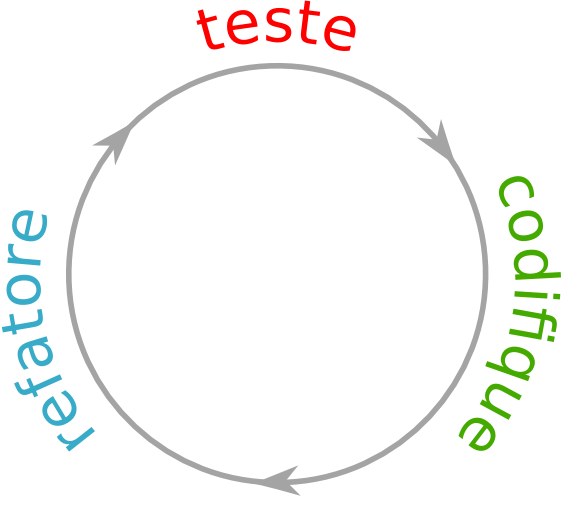
\includegraphics[scale=0.45]{images/ciclo-tdd}
  \label{img:ciclo-tdd}
\end{figure}

\subsection{TDD na prática}
\label{ssub:tdd_na_pratica}

Vejamos agora como isso se dá na prática através de um exemplo retirado do código do kanban-roots.

Precisa-se saber todas as tarefas em uma determinada posição do \textit{kanban} de um projeto. Então, a primeira coisa a ser feita é o teste para o caso mais simples: quando o projeto não tem tarefa alguma naquela determinada posição.

O teste para o caso mais simples pode ser como mostrado no código \ref{code:tdd_test1}.

\begin{mycode}{ruby}%
{Teste para o método Project\#tasks\_by\_position (versão 1)}{code:tdd_test1}
# test/unit/project_test.rb
class ProjectTest < ActiveSupport::TestCase
  def test_tasks_by_position
    project = Factory.create :project
    assert_equal(project.tasks_by_position(4), [])
  end
end
\end{mycode}

Ao rodar este teste, ele irá falhar, informando que o método \textit{tasks\_by\_position} sequer existe. Como esta era a falha esperada, escrevemos então o código mais simples para passar neste teste.

\begin{mycode}{ruby}%
{Código do método Project\#tasks\_by\_position (versão 1)}{code:tdd_code1}
# app/models/project.rb
def tasks_by_position position
  []
end
\end{mycode}

Os testes irão passar. Mas a funcionalidade ainda não está completa e, consequentemente, o teste também não.

\begin{mycode}{ruby}%
{Teste do método Project\#tasks\_by\_position (versão 2)}{code:tdd_test2}
# test/unit/project_test.rb
class ProjectTest < ActiveSupport::TestCase
  def test_tasks_by_position
    project = Factory.create :project
    tasks = [Factory.create(:task, :project => project, :position => 1),
             Factory.create(:task, :project => project, :position => 1)]

    assert_equal(project.tasks_by_position(4), [])

    assert_equal(project.tasks_by_position(1).count, 2)
    tasks.each { |task| assert(project.tasks_by_position(1).include?(task)) }
  end
end
\end{mycode}

O teste irá falhar, informando que na \hyperref[code:tdd_test1]{linha 9 do teste} eram esperadas duas tarefas, mas foram obtidas zero. O código então deve ser modificado para passar no novo teste.

\begin{mycode}{ruby}%
{Código do método Project\#tasks\_by\_position (versão 2)}{code:tdd_code2}
# app/models/project.rb
def tasks_by_position position
  task_list = []
  tasks.each do |task|
    task_list << task if task.position.to_s == position.to_s
  end
  task_list
end
\end{mycode}

Desta vez todos os testes os irão passar. Contudo, a cobertura de testes para este método ainda está fraca, o que pode ser resolvido com a adição de mais algumas tarefas em posições diferentes.

\begin{mycode}{ruby}%
{Teste do método Project\#tasks\_by\_position (versão 3)}{code:tdd_test3}
# test/unit/project_test.rb
class ProjectTest < ActiveSupport::TestCase
  def test_tasks_by_position
    project = Factory.create :project
    tasks = [Factory.create(:task, :project => project, :position => 1),
             Factory.create(:task, :project => project, :position => 1),
             Factory.create(:task, :project => project, :position => 2),
             Factory.create(:task, :project => project, :position => 3),
             Factory.create(:task, :project => project, :position => 3)]

    assert_equal(project.tasks_by_position(4), [])

    assert_equal(project.tasks_by_position(1).count, 2)
    tasks[0..1].each { |task| assert(project.tasks_by_position(1).include?(task)) }

    assert_equal(project.tasks_by_position(2), [tasks[2]])

    assert_equal(project.tasks_by_position(3).count, 2)
    tasks[3..4].each { |task| assert(project.tasks_by_position(3).include?(task)) }
  end
end
\end{mycode}

Executando os testes novamente, todos eles passam. Isto indica que já é hora de ir para o item 5 do ciclo TDD e refatorar. Ao comparar o Código \ref{code:tdd_code2} com o Código \ref{code:tdd_code3}, pode-se perceber como o Código \ref{code:tdd_code3} está mais simples e claro e que ao rodar os testes, estes passam mostrando que o comportamento do método não mudou.

\begin{mycode}{ruby}%
{Código do método Project\#tasks\_by\_position (versão 3)}{code:tdd_code3}
# app/models/project.rb
def tasks_by_position position
  tasks.select { |item| item.position.to_s == position.to_s }
end
\end{mycode}

\citeonline{TDDAntiPatterns} descreve vários anti-padrões do TDD e sua leitura é fortemente recomendada.


\section{Behaviour-Driven Development}

Criado em 2006 \cite{IntroducingBDD}, Behaviour-Driven Development (BDD) é uma técnica de desenvolvimento de software cuja amplitude se estende às atividades de design, documentação, validação e verificação, tratando-as de modo unificado \cite{BDDRodrigo}.

Como o nome já diz, Behaviour-Driven Development (Desenvolvimento guiado por comportamento) dá enfase no comportamento ao infez da estrutura. Ao invés de focar em classes e métodos ao escrever os testes, o foco é no comportamento que gera valor para o sistema.

Em TDD, o nome dos testes é baseado na estrutura do código, e isso pode ter um efeito colateral: cria duplicações. Ao escrever testes como o do Código \ref{code:tdd_test3} test\_tesks\_by\_position e o método tasks\_by\_position é renomeado, o nome do teste também terá que ser renomeado, o que provavelmente é esquecido. Isso torna os testes confusos e desinformativos \cite{ContinuousTesting}.

Por definição, refatorar é melhorar a estrutura e o design do código sem alterar seu comportamento. Nomeando os testes com base no comportamento desejado ao invés da estrutura do código, não apenas torna os testes mais informativos como também torna a refatoração menos custosa \cite{ContinuousTesting}. Pode-se ter a clara diferença comparando o Código \ref{code:tdd_test3} com o Código \ref{code:bdd_spec}.

\begin{mycode}{rspec}%
{Spec}{code:bdd_spec}
# spec/models/project.rb
describe Project do
  it "returns all related tasks matching a given position" do
    project = Factory.create :project
    tasks = [Factory.create(:task, :project => project, :position => 1),
             Factory.create(:task, :project => project, :position => 1),
             Factory.create(:task, :project => project, :position => 2),
             Factory.create(:task, :project => project, :position => 3),
             Factory.create(:task, :project => project, :position => 3)]

    project.tasks_by_position(4).should be_empty

    project.should have(2).tasks_by_position(1)
    project.tasks_by_position(1).should include(*tasks[0..1])

    project.tasks_by_position(2).should == [tasks[2]]

    project.should have(2).tasks_by_position(3)
    project.tasks_by_position(3).should include(*tasks[3..4])
  end
end
\end{mycode}

O BDD é uma evolução do TDD. A grande diferença entre os dois, é que TDD não abrange a validação do software, ou seja, se o software atende os requisitos. Isso muda tudo, pois em BDD, o pensamento não é voltado à verificação, mas sim no comportamento, em \textbf{validar} que o software faz o que deveria fazer, sem deixar também de \textbf{verificar} se está funcionando como deveria.

O Ciclo BDD é engloba o clico TDD visto anteriormente.

BDD vem se tornando um consenso em automação de testes. Contudo, existe controvérsia sobre seu modo de utilização.

Uma das maneiras de escrever testes de aceitação é como texto em língua humana,
ou seja, inglês, português e etc. Nestas ferramentas, os testes são escritos baseados em \textit{steps} (passos), onde os cada step é mapeado para um código real.

No código \ref{code:bdd_cucumber_spec}, é utilizado o cucumber para fazer a especificação de que os comentários devem ser renderizados utilizando a linguagem de marcação Markdown na página de tarefas. Como pode-se ver, o teste é escrito em linguagem que qualquer pessoa, mesmo sem nenhum conhecimento em programação, pode ler e validar. Este é um dos argumentos dos defensores da utilização dessa forma de escrita de testes, que o cliente pode validar os testes, inclusive ele mesmo escrevendo. Existem relatos de que na Globo.com esta abordagem é utilizada (procurar referências) e os clientes escrevem os testes.

\begin{mycode}{cucumber}%
{Especificação}{code:bdd_cucumber_spec}
# features/comments.feature
Feature: Render comments with Markdown syntax
  As a user
  I want to use Markdown in my comments
  In order to make my comments more expressives

  Scenario: on tasks page
    Given I am a contributor of "sgtran" project
    And I am authenticated
    And I have a task of "sgtran" project
    When I am on the task page
    And I fill in "comment_content" with "# Some content [link](http://exemplo.com)"
    And I press "Comment"
    Then I should see "Some content" in a "h1" tag
    And I should see "link" in an "a" tag
\end{mycode}

\begin{mycode}{rspec}%
{Especificação}{code:bdd_spec1}
# spec/acceptance/comments_spec.rb
feature "Render comments with Markdown syntax" do
  background do
    @owner = Factory.create :contributor
    @project = Factory.create :project
    @task = Factory.create :task, :project => @project, :author => @owner
  end

  scenario "on tasks page" do
    login(@owner.email, @owner.password)
    visit project_task_path(@project, @task)
    fill_in "comment_content", :with => "# Some content [link](http://exemplo.com)"
    click_button "Comment"
    page.should have_xpath("//h1", :text => "Some content")
    page.should have_xpath("//a", :text => "link", :href => "http://exemplo.com")
  end
end
\end{mycode}

\section{Integração contínua}

Em uma equipe com vários desenvolvedores, todos trabalhando na elaboração de um mesmo sistema, existe o problema de unificar as diversas alterações feitas na base de código, assegurando que a base continua consistente \cite{ImproveitCI}. Para resolver esse problema, entra em cena a Integração Contínua (IC), que além disso, tem como ponto chave dar um feedback rápido quando a base não está consistente.

\cite{FowlerCI} definiu a IC da seguinte maneira:

\begin{citacao}
Integração Contínua é uma prática de desenvolvimento de software onde os membros de um time integram seu trabalho frequentemente, geralmente cada pessoa integra ao menos uma vez ao dia - podendo haver múltiplas integrações por dia. Cada integração é verificada por um \textit{build} automatizado (incluindo testes) para detectar erros de integração o mais rápido possível. Muitos times acham que essa abordagem leva a uma significante redução nos problemas de integração e permite que um time desenvolva software coeso mais rapidamente.
\end{citacao}

A IC é um dos pilares da agilidade, pois garante que todo o sistema funcione de forma coesa a cada \textit{build}, mesmo que sua equipe seja grande e diversas partes do código estejam sendo alteradas ao mesmo tempo \cite{CaelumCI}.

Existe um debate sobre a periodicidade da integração, que tem relação direta com o tempo de execução da \textit{build}. Para assegurar o rápido feedback, esse tempo de execução deve ser o menor possível, tentando manter sempre menor do que dez minutos \cite{FowlerCI}.

\section{Teste contínuo}
\label{sub:teste_continuo}

Falar aqui de continuous testing.

\section{Dublês de Teste}

Em algumas ocasiões é difícil testar alguns componentes porque eles dependem de outros componentes que não podem ser utilizados em ambiente de teste. Estas situações podem acontecer por esses componentes não estarem disponíveis, por eles não retornam os resultados necessários ou porque executá-los iria trazer efeitos colaterais indesejados. Em outros casos, nossa estratégia de testes requer que nós tenhamos mais controle do comportamento interno do componente.

Quando estamos escrevendo um teste onde não podemos/escolhemos usar componentes reais, podemos substitui-los pelos Dublês de Teste que oferecem uma maneira de isolar as dependências ao criar seus testes, permitindo a utilização de componentes falsos para cumprir os papéis de componentes reais. Com isso, eliminamos complexidade do código dos testes, pois mantemos o código de implementação dos objetos pequeno e com baixo acoplamento.

Os Dublês de Teste não precisam se comportar exatamente como o componente real, eles devem apenas prover a mesma API que o componente real.

\citeonline{XUnit} Define cinco categorias de Dublês de Teste:

\begin{itemize}
\item
Objetos \textbf{\textit{Dummy}} geralmente são utilizados apenas para preencher uma lista de parâmetros e nunca são realmente usados.

\item
Objetos \textbf{\textit{Fake}} são utilizados para substituir funcionalidades reais de um componente por razões diferentes de verificações indiretas de entradas e saídas do componente a ser   testado.

\item
Os \textbf{\textit{Stubs}} provêm respostas prontas para chamadas feitas durante os testes, geralmente não respondendo a qualquer   chamada diferente
das pré-definidas.

\item
Os \textbf{\textit{Spies}} são \textit{Stubs} que também tem gravam algumas informações baseadas em como eles são chamados. Um exemplo   pode ser um serviço de email que grava quantas mensagens foram   enviadas.

\item
\textbf{\textit{Mocks}} são objetos pré-programados para receber determinado conjunto de chamadas, podendo lançar uma exceção se tais chamadas não forem feitas a ele, ou se receber outra chamada diferente das pré-programadas.
\end{itemize}

De modo geral, a utilização de Dublês de Teste é extremamente benéfica para o projeto. Contudo, existem controvérsias, principalmente em relação a utilização do \textit{Mock} \cite{MocksArentStubs}.